% =============================================================
% บทที่ 4 - ผลการดำเนินงานและผลการวิเคราะห์
% ตัวเลขทุกค่าในบทนี้มาจากการรันโค้ดใน money-printer-research:
%   - notebooks/hypothesis_1.ipynb, hypothesis_2.ipynb (หัวข้อ 4.1)
%   - notebooks/match_features_eda.ipynb, uv run feature_importance (หัวข้อ 4.2)
%   - uv run learning_curve, notebooks/model_comparison.ipynb (หัวข้อ 4.3)
%   - data/predictions/backtest.csv (หัวข้อ 4.4)
%   - uv run report (analysis.json, code 7ced6ad, strategies.toml 1521070) (หัวข้อ 4.5--4.7)
% =============================================================

บทนี้เสนอผลการดำเนินงานตามลำดับของกระบวนการวิทยาการข้อมูล ได้แก่ ผลการทดสอบสมมติฐานทางสถิติ ผลการสำรวจและคัดเลือกตัวแปร ผลการประเมินแบบจำลองทำนายผล ผลการทดสอบย้อนหลังของแบบจำลอง ผลการเปรียบเทียบกับตลาดเดิมพันและชุดกลยุทธ์ที่ลงทะเบียนไว้ล่วงหน้า ผลของกลยุทธ์การบริหารเงินทุน และความเป็นไปได้ในการนำไปใช้จริง ตัวเลขทุกค่าในบทนี้ได้จากการรันโค้ดของโครงงานบนข้อมูลจริง และสามารถสร้างซ้ำได้จากรหัสคอมมิตที่ระบุไว้ในรายงาน

% -----------------------------------------------------------
\section{ผลการทดสอบสมมติฐานทางสถิติ}
% -----------------------------------------------------------

การทดสอบในหัวข้อนี้ใช้ข้อมูลพรีเมียร์ลีกอังกฤษตั้งแต่ฤดูกาล 2000--2001 ถึง 2024--2025 ที่มีคะแนน Elo ก่อนแข่งครบทั้งสองทีม โดยตัดนัดในช่วง 28 วันแรกของแต่ละฤดูกาลออก เนื่องจากคะแนน Elo ของทีมที่เลื่อนชั้นยังไม่เข้าที่ คงเหลือ 8,469 นัด จากทั้งหมด 9,380 นัด และใช้ระดับนัยสำคัญ $\alpha = 0.05$

\subsection{ความได้เปรียบของการเป็นเจ้าบ้าน (Home Advantage)}

กำหนดสมมติฐาน $H_0: \mu_d = 0$ และ $H_1: \mu_d > 0$ เมื่อ $\mu_d$ คือค่าเฉลี่ยของผลต่างประตู (ประตูเจ้าบ้าน $-$ ประตูทีมเยือน) ต่อนัด ผลการทดสอบแสดงดังตารางที่ \ref{tab:home_advantage}

\begin{table}[htbp]
\centering
\caption{ผลการทดสอบความได้เปรียบของทีมเจ้าบ้าน (พรีเมียร์ลีก 8,469 นัด)}
\label{tab:home_advantage}
\begin{tabular}{|l|c|}
\hline
\textbf{รายการ} & \textbf{ค่าที่ได้} \\
\hline
ค่าเฉลี่ยประตูทีมเจ้าบ้านต่อนัด & $1.541$ \\
ค่าเฉลี่ยประตูทีมเยือนต่อนัด & $1.179$ \\
ผลต่างเฉลี่ย ($\bar{d}$) & $+0.362$ \\
Paired t-test (one-sided) & $t = 18.35$, $p = 4.39 \times 10^{-74}$ \\
Wilcoxon Signed-rank Test (one-sided) & $p = 3.75 \times 10^{-75}$ \\
\hline
\end{tabular}
\end{table}

ทั้งสองวิธีปฏิเสธ $H_0$ ที่ระดับนัยสำคัญ $0.05$ ทีมเจ้าบ้านทำประตูได้มากกว่าทีมเยือนเฉลี่ย $0.362$ ประตูต่อนัด ผลนี้สนับสนุนการกำหนดค่าความได้เปรียบของเจ้าบ้าน ($h = 40$ คะแนน) ในระบบ Elo Rating ตามที่อธิบายไว้ในบทที่ 3

\subsection{ความสัมพันธ์ระหว่างผลต่างคะแนน Elo กับผลต่างประตู}

กำหนดสมมติฐาน $H_0: \beta = 0$ (ผลต่างคะแนน Elo ไม่มีความสัมพันธ์เชิงเส้นกับผลต่างประตู) และ $H_1: \beta \neq 0$ ผลการวิเคราะห์บนชุดข้อมูลเดียวกันพบว่า

\begin{itemize}
    \item สัมประสิทธิ์สหสัมพันธ์ของ Pearson $r = 0.441$ และของ Spearman $\rho = 0.429$ โดย $p$-value ของทั้งสองค่าต่ำกว่าความละเอียดของการคำนวณ ($p \approx 0$) จึงปฏิเสธ $H_0$ ผลต่างคะแนน Elo มีความสัมพันธ์เชิงบวกระดับปานกลางกับผลต่างประตู
    \item ในกลุ่มนัดที่สองทีมมีคะแนนใกล้เคียงกัน ($|\Delta R| < 25$) จำนวน 1,406 นัด ทีมเจ้าบ้านยังมีผลต่างประตูเฉลี่ย $+0.394$ ประตู ($t = 9.20$, $p = 1.2 \times 10^{-19}$) แสดงว่าความได้เปรียบของเจ้าบ้านยังคงอยู่แม้ความแข็งแกร่งของสองทีมเท่ากัน
\end{itemize}

% -----------------------------------------------------------
\section{ผลการสำรวจและคัดเลือกตัวแปร}
% -----------------------------------------------------------

ตารางตัวแปรรายนัด (\texttt{match\_features}) ของ 5 ลีกมี 21,882 นัด และตัวแปรก่อนแข่ง 140 คอลัมน์ ผลลัพธ์หลังจบเกม เช่น ประตูและ xG ของนัดนั้น ถูกกันออกจากรายชื่อตัวแปรที่อนุญาต (Allowlist) จึงไม่สามารถรั่วเข้าสู่แบบจำลองได้ การสำรวจใช้เฉพาะชุดฝึก (18,085 นัด 10 ฤดูกาล) โดยไม่เปิดดูนัดตั้งแต่ฤดูกาล 2024--2025 (3,797 นัด) ชุดทดสอบใช้เฉพาะฤดูกาลที่แข่งจบแล้ว คือ 2024--2025 และ 2025--2026 ส่วน 293 นัดของฤดูกาล 2026--2027 ที่ยังแข่งไม่จบไม่ถูกใช้วัดผล เพราะเป็นเพียงช่วงต้นฤดูกาลและยังไม่มีข้อมูลตารางแข่งจาก Transfermarkt

\subsection{สัดส่วนผลการแข่งขันในแต่ละฤดูกาล}

ภาพที่ \ref{fig:outcome_shares} แสดงสัดส่วนเจ้าบ้านชนะ (H) เสมอ (D) และทีมเยือนชนะ (A) ของแต่ละลีกในชุดฝึก เจ้าบ้านชนะประมาณร้อยละ 39--49 ในฤดูกาลปกติ ยกเว้นฤดูกาล 2020--2021 (แถบสีเทา) ที่แข่งขันโดยไม่มีผู้ชมเนื่องจากการระบาดของ COVID-19 สัดส่วนเจ้าบ้านชนะลดลงเหลือร้อยละ 37--42 และในพรีเมียร์ลีกทีมเยือนชนะ (ร้อยละ 40.3) มากกว่าเจ้าบ้านชนะ (ร้อยละ 37.9) สัดส่วนผลจึงเปลี่ยนไปตามฤดูกาลและลีก การทายจากสัดส่วนผล (Class Prior) ที่ใช้เป็นเกณฑ์ขั้นต่ำจึงคำนวณจากฤดูกาลก่อนหน้าเท่านั้น

\begin{figure}[H]
    \centering
    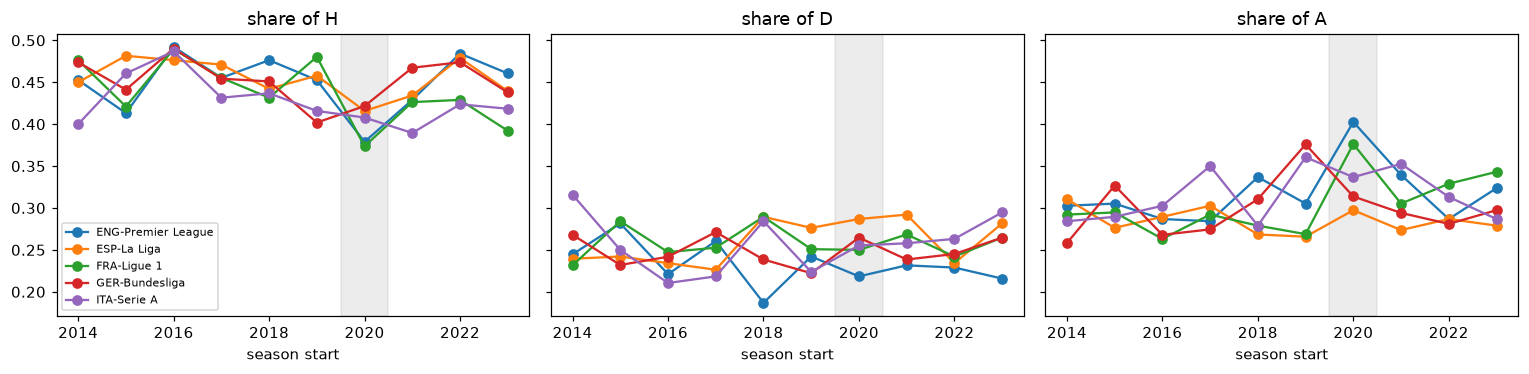
\includegraphics[width=\textwidth]{images/outcome_shares.png}
    \caption{สัดส่วนผล H/D/A ของแต่ละลีกตามฤดูกาล (ชุดฝึก แถบสีเทาคือฤดูกาล 2020--2021)}
    \label{fig:outcome_shares}
\end{figure}

\subsection{ความสัมพันธ์ของตัวแปรแต่ละตัวกับผลการแข่งขัน}

ภาพที่ \ref{fig:feature_deciles} แบ่งตัวแปรผลต่าง (ทีมเจ้าบ้าน $-$ ทีมเยือน) แต่ละตัวออกเป็น 10 ช่วงเท่ากัน แล้วแสดงสัดส่วนเจ้าบ้านชนะ (H) เสมอ (D) และทีมเยือนชนะ (A) ในแต่ละช่วง เส้นที่ชันแสดงว่าตัวแปรนั้นเปลี่ยนโอกาสของผลการแข่งขัน ส่วนเส้นที่แบนแสดงว่าตัวแปรนั้นแทบไม่บอกอะไร

\begin{figure}[H]
    \centering
    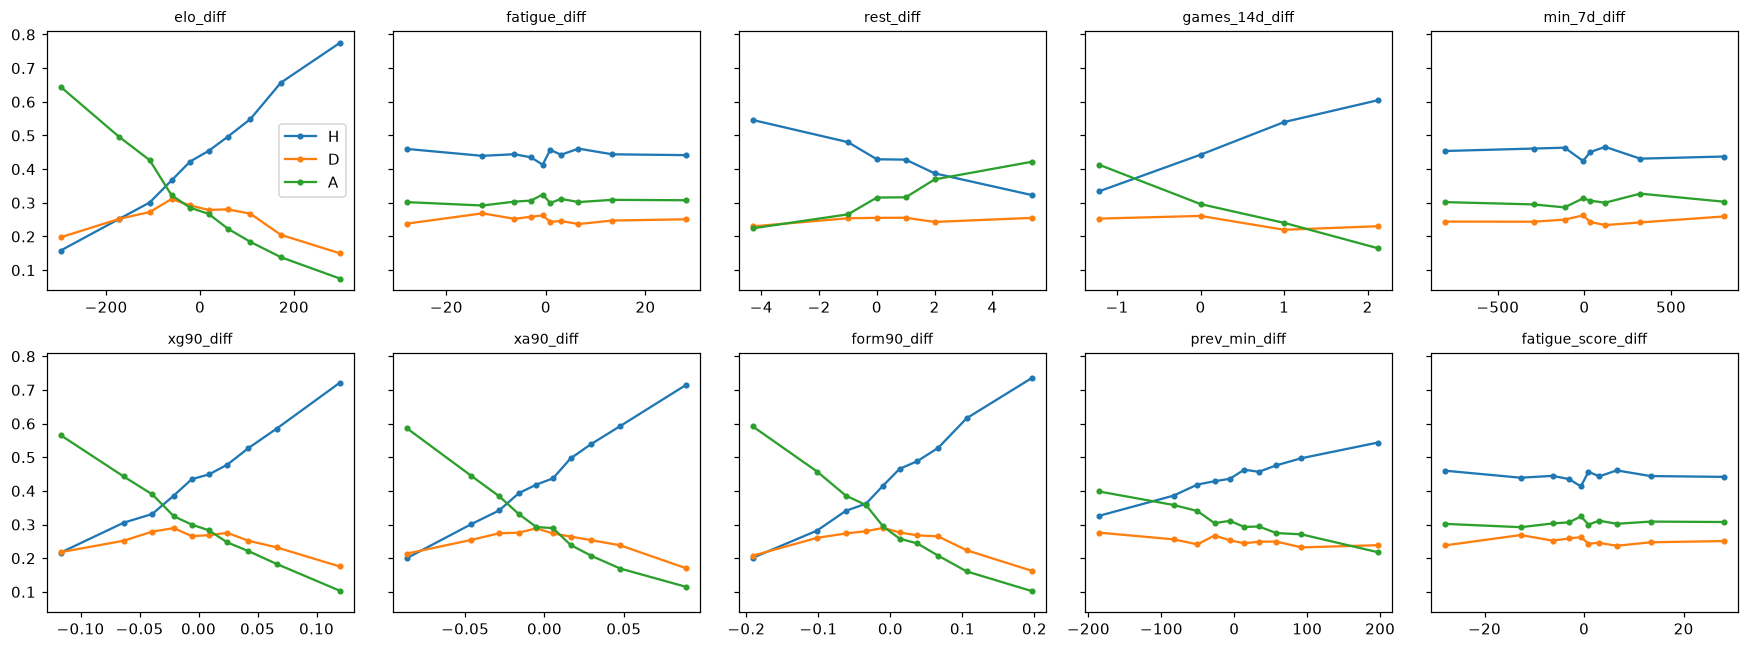
\includegraphics[width=\textwidth]{images/feature_deciles.png}
    \caption{สัดส่วนผล H/D/A ตามช่วงเดไซล์ของตัวแปรผลต่างก่อนแข่งแต่ละตัว (ชุดฝึก)}
    \label{fig:feature_deciles}
\end{figure}

ผลต่างคะแนน Elo ให้ความชันมากที่สุด โอกาสเจ้าบ้านชนะเปลี่ยนจากประมาณ $0.16$ ในช่วงต่ำสุดเป็น $0.78$ ในช่วงสูงสุด (ช่วงห่าง $0.62$) ตามด้วยฟอร์มผู้เล่นตัวจริง \texttt{form90} ($0.53$) \texttt{xa90} ($0.51$) และ \texttt{xg90} ($0.50$) ในทางกลับกัน ดัชนีความเหนื่อยล้า (\texttt{fatigue\_diff}) และนาทีที่ลงเล่นใน 7 วัน (\texttt{min\_7d\_diff}) ให้เส้นเกือบแบน (ช่วงห่างไม่ถึง $0.05$)

\subsection{ความซ้ำซ้อนระหว่างตัวแปร}

ภาพที่ \ref{fig:feature_correlation} แสดงค่าสหสัมพันธ์ระหว่างตัวแปรหลักบน 16,242 นัดที่มีครบทุกตัว พบว่า \texttt{fatigue\_score\_diff} กับ \texttt{fatigue\_diff} เป็นตัวแปรเดียวกัน ($r = 1.00$) \texttt{fatigue\_diff} กับ \texttt{min\_7d\_diff} เคลื่อนไหวไปด้วยกัน ($r = 0.93$) และ \texttt{form90\_diff} ครอบคลุมทั้ง \texttt{xg90\_diff} ($r = 0.95$) และ \texttt{xa90\_diff} ($r = 0.91$) จึงควรเลือกใช้เพียงตัวเดียวในแต่ละกลุ่ม นอกจากนี้ \texttt{form90\_diff} มีสหสัมพันธ์กับ \texttt{elo\_diff} สูงถึง $0.73$

\begin{figure}[H]
    \centering
    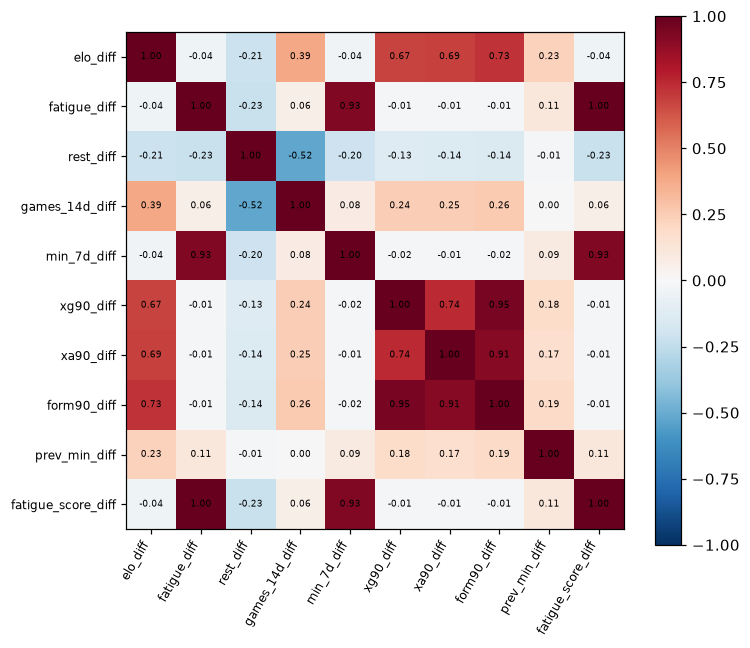
\includegraphics[width=0.75\textwidth]{images/feature_correlation.png}
    \caption{เมทริกซ์สหสัมพันธ์ของตัวแปรผลต่างหลัก (16,242 นัด)}
    \label{fig:feature_correlation}
\end{figure}

เพื่อตรวจว่าตัวแปรอื่นให้ข้อมูลเพิ่มจากคะแนน Elo จริงหรือไม่ ได้เปรียบเทียบ Logistic Regression ที่ใช้ \texttt{elo\_diff} อย่างเดียว (Log Loss $0.9740$) กับที่เพิ่มตัวแปรครั้งละหนึ่งตัว โดยฝึกด้วยฤดูกาล 2015--2022 และวัดผลบนฤดูกาล 2023 ของชุดฝึก (ใช้เฉพาะนัดที่มีค่าครบทั้งสองตัวแปร ประมาณ 16,250 นัด) ค่าในตารางนี้จึงไม่ใช่ค่าเดียวกับ Log Loss แบบ Walk-forward ในตารางที่ \ref{tab:forward_selection} ผลแสดงดังตารางที่ \ref{tab:gain_over_elo}

\begin{table}[htbp]
\centering
\caption{Log Loss บนฤดูกาล 2023 ที่ลดลงเมื่อเพิ่มตัวแปรหนึ่งตัวเข้าไปในแบบจำลองที่มีคะแนน Elo อยู่แล้ว}
\label{tab:gain_over_elo}
\begin{tabular}{|l|c|c|}
\hline
\textbf{ตัวแปรที่เพิ่ม} & \textbf{Log Loss (Elo + ตัวแปร)} & \textbf{ส่วนที่ลดลง} \\
\hline
\texttt{form90\_diff} & $0.97002$ & $+0.00395$ \\
\texttt{xa90\_diff} & $0.97010$ & $+0.00387$ \\
\texttt{xg90\_diff} & $0.97161$ & $+0.00236$ \\
\texttt{games\_14d\_diff} & $0.97401$ & $-0.00006$ \\
\texttt{rest\_diff} & $0.97405$ & $-0.00009$ \\
\texttt{fatigue\_diff} & $0.97411$ & $-0.00015$ \\
\texttt{prev\_min\_diff} & $0.97419$ & $-0.00023$ \\
\texttt{min\_7d\_diff} & $0.97437$ & $-0.00041$ \\
\hline
\end{tabular}
\end{table}

มีเพียงฟอร์มผู้เล่นตัวจริงเท่านั้นที่ช่วยลด Log Loss ได้เมื่อมีคะแนน Elo อยู่แล้ว ตัวแปรด้านความเหนื่อยล้าและตารางแข่งในรูปผลต่าง กลับทำให้แบบจำลองแย่ลงเล็กน้อย ส่วนหนึ่งเป็นเพราะสโมสรใหญ่ที่มีคะแนน Elo สูงมักเป็นทีมที่ลงแข่งรายการยุโรปและมีตารางแข่งหนาแน่น ข้อมูลตารางแข่งจึงซ้ำกับสิ่งที่ Elo บอกอยู่แล้ว

\subsection{การคัดเลือกตัวแปรแบบเดินหน้า (Forward Selection)}

การคัดเลือกตัวแปรขั้นสุดท้ายทำบนตารางสำหรับฝึกแบบจำลอง 20,054 นัด และ 18 กลุ่มตัวแปร โดยเริ่มจากคะแนน Elo แล้วเพิ่มกลุ่มที่ลด Log Loss แบบ Walk-forward บนฤดูกาล 2021--2023 ได้มากที่สุดทีละกลุ่ม จนไม่มีกลุ่มใดลดได้เกินเกณฑ์ขั้นต่ำ ผลแสดงดังตารางที่ \ref{tab:forward_selection}

\begin{table}[htbp]
\centering
\caption{ผลการคัดเลือกกลุ่มตัวแปรแบบเดินหน้า (Walk-forward Log Loss ฤดูกาล 2021--2023)}
\label{tab:forward_selection}
\small
\begin{tabular}{|c|l|l|c|c|}
\hline
\textbf{ลำดับ} & \textbf{กลุ่มตัวแปรที่เพิ่ม} & \textbf{ความหมาย} & \textbf{Log Loss} & \textbf{ส่วนที่ลดลง} \\
\hline
1 & \texttt{elo} & คะแนน Elo ก่อนแข่ง & $0.9842$ & -- \\
2 & \texttt{player\_form90} & ฟอร์มผู้เล่นตัวจริงต่อ 90 นาที & $0.9828$ & $0.0014$ \\
3 & \texttt{games\_14d\_all} & จำนวนนัดทุกรายการใน 14 วัน & $0.9818$ & $0.0010$ \\
4 & \texttt{player\_prev\_min} & นาทีที่ผู้เล่นตัวจริงลงเล่นก่อนหน้า & $0.9811$ & $0.0007$ \\
\hline
\end{tabular}
\end{table}

เมื่อนำไปวัดผลครั้งเดียวบนชุดทดสอบ (ฤดูกาล 2024--2025 และ 2025--2026) ได้ผลดังตารางที่ \ref{tab:feature_holdout} ชุดตัวแปรที่คัดเลือกดีกว่าการใช้ Elo อย่างเดียว และดีกว่าการใส่ทุกกลุ่มตัวแปร ซึ่งยืนยันว่ากลุ่มที่ไม่ถูกเลือก (รวมถึงดัชนีความเหนื่อยล้า วันพัก และแผนการเล่น) เพิ่มแต่สัญญาณรบกวน

\begin{table}[htbp]
\centering
\caption{Log Loss บนชุดทดสอบ (ฤดูกาล 2024--2025 และ 2025--2026) ตามชุดตัวแปร}
\label{tab:feature_holdout}
\begin{tabular}{|l|c|}
\hline
\textbf{ชุดตัวแปร} & \textbf{Log Loss} $\downarrow$ \\
\hline
ทายจากสัดส่วนผลอย่างเดียว (Class Prior) & $1.0749$ \\
คะแนน Elo อย่างเดียว & $0.9893$ \\
\textbf{ชุดตัวแปรที่คัดเลือก (4 กลุ่ม)} & $\mathbf{0.9855}$ \\
ทุกกลุ่มตัวแปร (18 กลุ่ม) & $0.9879$ \\
\hline
\end{tabular}
\end{table}

% -----------------------------------------------------------
\section{ผลการประเมินประสิทธิภาพของแบบจำลอง}
% -----------------------------------------------------------

แบบจำลองทั้ง 4 แบบใช้ชุดตัวแปรที่คัดเลือกชุดเดียวกัน ได้แก่ Logistic Regression แบบหลายกลุ่ม (Multinomial), Logistic Regression ที่ปรับเทียบความน่าจะเป็นด้วย Sigmoid, Gradient-boosted Trees และแบบจำลองจำนวนประตู Poisson (Poisson Regression หนึ่งตัวต่อหนึ่งฝั่ง แล้วรวมตารางสกอร์เป็นความน่าจะเป็น H/D/A) ทุกแบบจำลองฝึกด้วยข้อมูลก่อนฤดูกาล 2024--2025 (16,258 นัด) และวัดผลบนชุดทดสอบชุดเดียวกัน คือ 3,503 นัดของฤดูกาล 2024--2025 และ 2025--2026 ในตารางสำหรับฝึกแบบจำลอง (20,054 นัด) ทุกนัดมีราคาต่อรอง จึงวัดราคาเจ้ามือบนนัดชุดเดียวกันได้

\subsection{เส้นโค้งการเรียนรู้ (Learning Curve)}

ภาพที่ \ref{fig:learning_curve} แสดง Log Loss บนชุดทดสอบเมื่อฝึกด้วยนัดล่าสุดจำนวนต่าง ๆ ตั้งแต่ 250 นัดจนถึงทั้งหมด 16,258 นัด เส้นประด้านบนคือการทายจากสัดส่วนผลอย่างเดียว ($1.0749$) และเส้นประด้านล่างคือความน่าจะเป็นจากราคาเจ้ามือบนนัดชุดเดียวกัน ($0.9691$)

\begin{figure}[H]
    \centering
    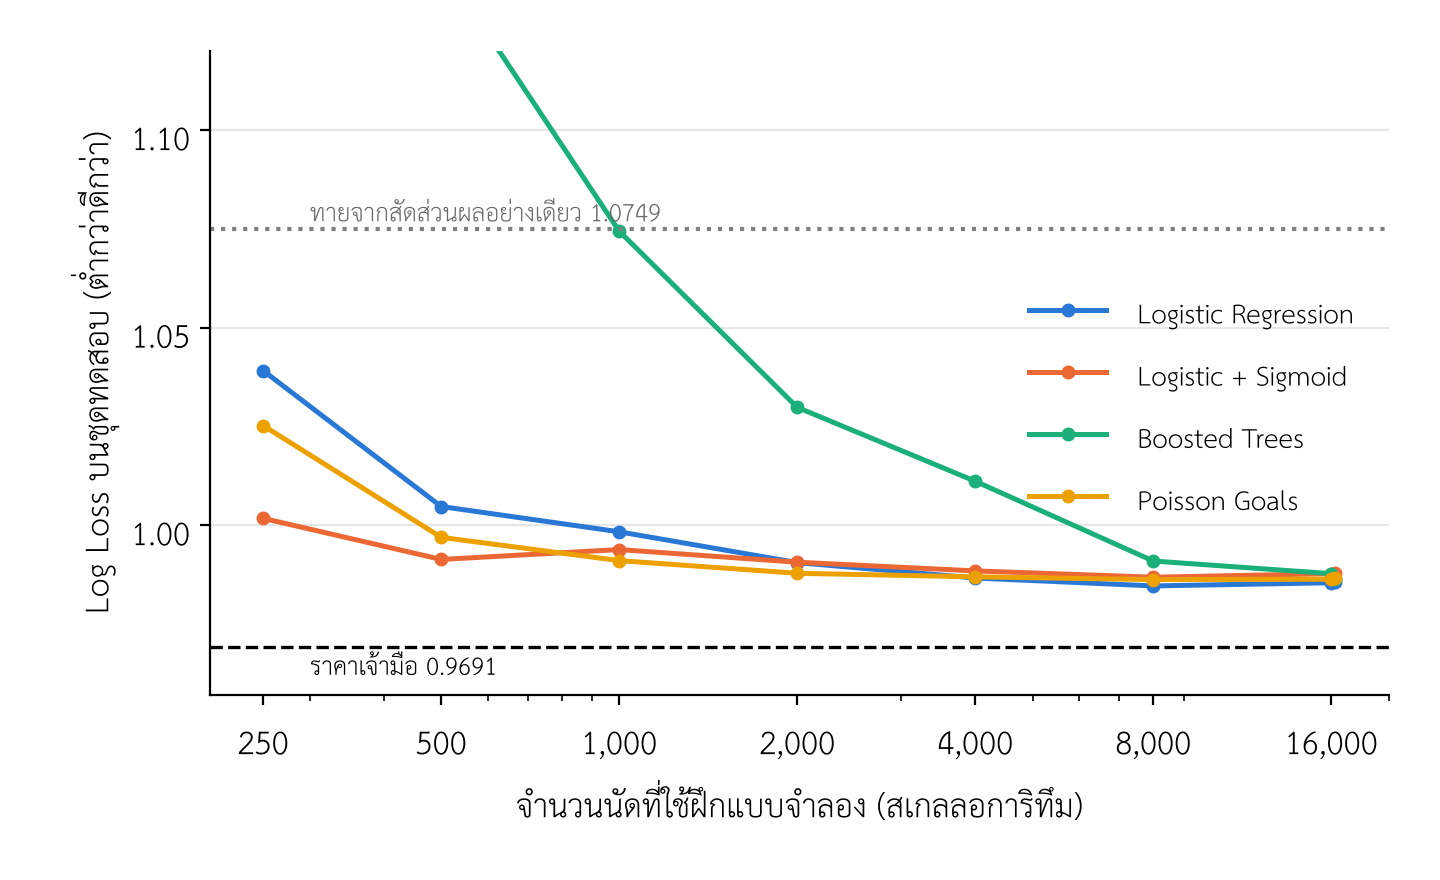
\includegraphics[width=0.9\textwidth]{images/learning_curve.png}
    \caption{Log Loss บนชุดทดสอบเทียบกับจำนวนนัดที่ใช้ฝึกของแบบจำลองทั้ง 4 แบบ}
    \label{fig:learning_curve}
\end{figure}

ผลที่สำคัญมีดังนี้
\begin{enumerate}[label=\arabic*)]
    \item Logistic Regression ให้ผลดีที่สุดที่ $0.9846$ ($\pm 0.0081$) เมื่อฝึกด้วย 8,000 นัด และ $0.9855$ เมื่อฝึกด้วยทุกนัด เส้นแบนตั้งแต่ประมาณ 4,000 นัด การเพิ่มข้อมูลเท่าตัวในรอบสุดท้ายไม่ช่วยลด Log Loss เลย
    \item เมื่อฝึกด้วยทุกนัด Log Loss บนชุดฝึก ($0.9791$) กับชุดทดสอบ ($0.9855$) ห่างกันเพียง $0.0064$ แสดงว่าแบบจำลองไม่ได้จำข้อมูล (Overfitting) แต่เรียนรู้ได้เต็มที่เท่าที่ชุดตัวแปรนี้ให้ได้แล้ว
    \item Gradient-boosted Trees ต้องการข้อมูลมากที่สุด ที่ 250 นัดได้ Log Loss $1.2623$ ซึ่งแย่กว่าการทายจากสัดส่วนผล และไล่ตาม Logistic Regression ได้เมื่อใช้ข้อมูลทั้งหมดเท่านั้น
    \item Logistic Regression ที่ฝึกด้วยทุกนัด ($0.9855$) ยังด้อยกว่าราคาเจ้ามือ ($0.9691$) อยู่ $0.0164$ (และ $0.0155$ แม้ที่จุดดีที่สุด 8,000 นัด) ซึ่งมากกว่าช่วงความคลาดเคลื่อนมาตรฐาน หมายความว่าข้อมูลสาธารณะชุดนี้ไม่พอให้ทำนายได้แม่นเท่าตลาด
\end{enumerate}

\subsection{เปรียบเทียบตัวชี้วัดหลายมิติ}

ตารางที่ \ref{tab:model_comparison} สรุปผลเมื่อฝึกด้วยข้อมูลทั้งหมดก่อนฤดูกาล 2024--2025 พร้อม RPS, Brier Score และ Accuracy จาก \texttt{uv run modeling}

\begin{table}[htbp]
\centering
\caption{ประสิทธิภาพของแบบจำลองบนชุดทดสอบ (ฤดูกาล 2024--2025 และ 2025--2026, 3,503 นัด)}
\label{tab:model_comparison}
\small
\begin{tabular}{|l|c|c|c|c|}
\hline
\textbf{แบบจำลอง} & \textbf{Log Loss} $\downarrow$ & \textbf{RPS} $\downarrow$ & \textbf{Brier} $\downarrow$ & \textbf{Accuracy} $\uparrow$ \\
\hline
ทายจากสัดส่วนผล (Class Prior) & $1.0749$ & -- & -- & -- \\
\textbf{Logistic Regression} & $\mathbf{0.9855}$ & $0.2005$ & $\mathbf{0.5875}$ & $\mathbf{52.41\%}$ \\
Poisson Goals & $0.9865$ & $\mathbf{0.2004}$ & $0.5880$ & $52.18\%$ \\
Gradient-boosted Trees & $0.9876$ & $0.2010$ & $0.5886$ & $51.98\%$ \\
Logistic + Sigmoid & $0.9877$ & $0.2007$ & $0.5888$ & $52.41\%$ \\
\hline
ราคาเจ้ามือ (อ้างอิง) & $0.9691$ & -- & -- & $54.1\%$ \\
\hline
\end{tabular}
\end{table}

ความแตกต่างระหว่างแบบจำลองทั้ง 4 แบบน้อยกว่าช่วงความคลาดเคลื่อนมาตรฐาน ($\approx 0.008$) แต่ Logistic Regression ดีที่สุดหรือใกล้เคียงที่สุดในทุกตัวชี้วัด และเรียบง่ายที่สุด จึงถูกเลือกเป็นแบบจำลองหลักสำหรับการทดสอบย้อนหลังและการทำนายนัดที่กำลังจะมาถึง Gradient Boosting ซึ่งนำมาเพื่อตรวจหาความสัมพันธ์ไม่เชิงเส้น (บทที่ 3) ไม่ได้ให้ผลดีกว่า แสดงว่าสัญญาณของตัวแปรส่วนใหญ่เป็นเชิงเส้น และเมื่อข้อมูลฝึกมีน้อย Gradient Boosting จะเรียนรู้สัญญาณรบกวนจนแย่กว่าการทายจากสัดส่วนผล (ภาพที่ \ref{fig:learning_curve}) นอกจากนี้ Accuracy ที่ $52.41\%$ สูงกว่าช่วง $47.84$--$48.60\%$ ของแบบจำลองที่ใช้เพียงผลสกอร์ย้อนหลังที่ Hubáček และคณะ \cite{hubacek2021forty} รายงานไว้ (คนละชุดข้อมูล จึงเทียบได้เพียงคร่าว ๆ) แต่ต่ำกว่าการทายทีมต่อตามราคาปิดของ Pinnacle ซึ่งถูก $54.1\%$ บนนัดทดสอบชุดเดียวกัน (3,503 นัด)

% -----------------------------------------------------------
\section{ผลการทดสอบย้อนหลังของแบบจำลอง (Model Backtest)}
% -----------------------------------------------------------

การทดสอบย้อนหลังทำนายแต่ละฤดูกาลตั้งแต่ 2017--2018 ถึง 2025--2026 ด้วย Logistic Regression ที่ฝึกจากฤดูกาลก่อนหน้าเท่านั้น (Walk-forward) รวม 16,110 นัด (ไม่รวมนัดของฤดูกาล 2026--2027 ที่เริ่มแข่งแล้ว) แต่ละนัดเลือกผลที่มีค่าคาดหมายสูงสุด $EV = p \times \text{Odds} - 1$ แล้ววางเดิมพัน 1 หน่วยที่ราคาปิดของ Pinnacle เมื่อ $EV$ สูงกว่าเกณฑ์ ผลแสดงดังตารางที่ \ref{tab:backtest_threshold} และภาพที่ \ref{fig:backtest_cumulative}

\begin{table}[htbp]
\centering
\caption{ผลการวางเดิมพันตามแบบจำลองที่เกณฑ์ $EV$ ต่าง ๆ (ฤดูกาล 2017--2025, เดิมพันละ 1 หน่วย)}
\label{tab:backtest_threshold}
\begin{tabular}{|c|r|c|r|c|}
\hline
\textbf{เกณฑ์ $EV$} & \textbf{จำนวนเดิมพัน} & \textbf{อัตราชนะ} & \textbf{กำไรสุทธิ (หน่วย)} & \textbf{ROI} \\
\hline
$> 0\%$ & 15,352 & $34.5\%$ & $-665.2$ & $-4.33\%$ \\
$> 2\%$ & 14,127 & $33.7\%$ & $-661.0$ & $-4.68\%$ \\
$> 5\%$ & 12,032 & $32.2\%$ & $-661.3$ & $-5.50\%$ \\
$> 10\%$ & 8,928 & $30.5\%$ & $-407.2$ & $-4.56\%$ \\
$> 20\%$ & 4,728 & $26.5\%$ & $-226.7$ & $-4.80\%$ \\
\hline
\end{tabular}
\end{table}

\begin{figure}[H]
    \centering
    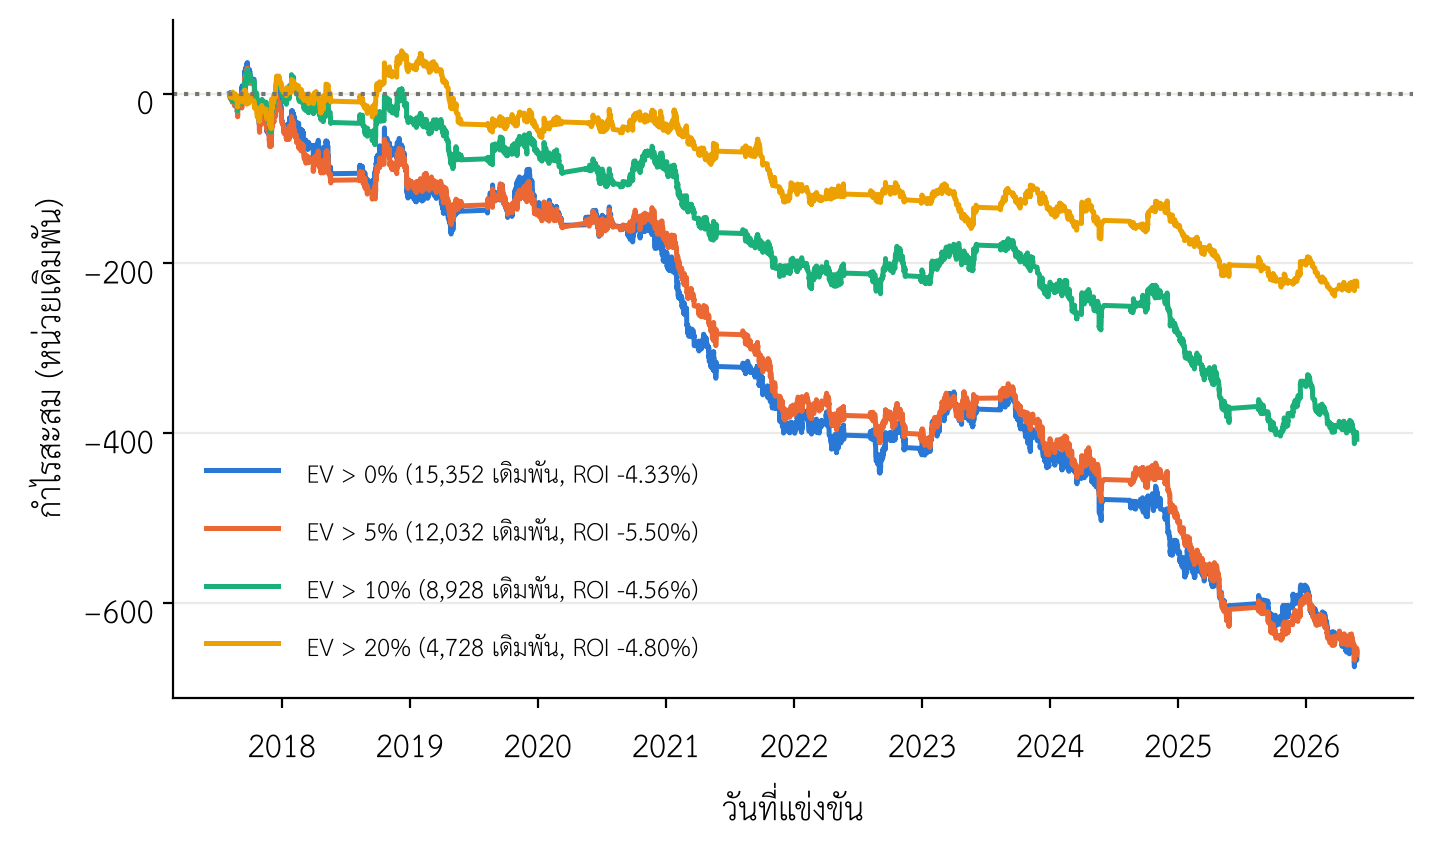
\includegraphics[width=0.9\textwidth]{images/backtest_cumulative.png}
    \caption{กำไรสะสมจากการวางเดิมพันตามแบบจำลองที่เกณฑ์ $EV$ ต่าง ๆ}
    \label{fig:backtest_cumulative}
\end{figure}

ทุกเกณฑ์ขาดทุนในอัตราใกล้เคียงกันประมาณ $4$--$5.5\%$ การเพิ่มเกณฑ์ $EV$ ไม่ได้ทำให้ผลดีขึ้น แสดงว่า $EV$ ที่สูงตามแบบจำลองส่วนใหญ่มาจากความคลาดเคลื่อนของแบบจำลองเอง ไม่ใช่ความผิดพลาดของตลาด เมื่อแยกรายฤดูกาล มีเพียงฤดูกาล 2022 ที่ได้กำไร ($+30.7$ หน่วย, ROI $+1.74\%$) ส่วนอีก 8 ฤดูกาลขาดทุน และเมื่อแยกรายลีก มีเพียงบุนเดสลีกาที่ ROI เป็นบวกเล็กน้อย ($+0.49\%$ จาก 2,640 เดิมพัน) ซึ่งอยู่ในช่วงที่เกิดได้จากความบังเอิญ

% -----------------------------------------------------------
\section{ผลการเปรียบเทียบกับตลาดเดิมพัน}
% -----------------------------------------------------------

เนื่องจากแบบจำลองที่ใช้ข้อมูลทีมอย่างเดียวด้อยกว่าราคาตลาด การวิเคราะห์ส่วนนี้จึงตั้งคำถามที่เข้มงวดขึ้น คือ ถ้าเริ่มจากราคาตลาดแล้วเพิ่มข้อมูลทีมเข้าไป จะทำนายได้ดีกว่าตลาดหรือไม่ โดยใช้ข้อมูลจาก Football-Data.co.uk 20,712 นัดของ 5 ลีก ฤดูกาล 2014--2015 ถึง 2025--2026 และวัดผล 17,063 นัดตั้งแต่ฤดูกาล 2016--2017 ทุกฤดูกาลทำนายจากฤดูกาลก่อนหน้าเท่านั้น ผลแสดงดังตารางที่ \ref{tab:market_forecasters} และ \ref{tab:market_diff}

\begin{table}[htbp]
\centering
\caption{คะแนนเฉลี่ยของผู้ทำนายแต่ละแบบบนนัดชุดเดียวกัน 17,063 นัด}
\label{tab:market_forecasters}
\begin{tabular}{|l|c|c|}
\hline
\textbf{ผู้ทำนาย (Forecaster)} & \textbf{Log Loss} $\downarrow$ & \textbf{RPS} $\downarrow$ \\
\hline
ราคาปิดของ Pinnacle (Closing Price) & $\mathbf{0.9608}$ & $\mathbf{0.1932}$ \\
ราคาเปิดของ Pinnacle (Early Price) & $0.9632$ & $0.1938$ \\
ราคาเปิดที่ปรับเทียบใหม่ (Recalibrated) & $0.9637$ & $0.1940$ \\
ราคาเปิด + ฟอร์มทีม & $0.9641$ & $0.1940$ \\
ฟอร์มทีมอย่างเดียว & $0.9805$ & $0.1989$ \\
\hline
\end{tabular}
\end{table}

\begin{table}[htbp]
\centering
\caption{ผลต่าง Log Loss แบบจับคู่รายนัด (ค่าติดลบหมายถึงผู้ทำนายตัวแรกดีกว่า)}
\label{tab:market_diff}
\begin{tabular}{|l|c|c|}
\hline
\textbf{การเปรียบเทียบ} & \textbf{ผลต่าง} & \textbf{ช่วงความเชื่อมั่น 95\%} \\
\hline
ราคาปิด เทียบ ราคาเปิด & $-0.0024$ & $-0.0035$ ถึง $-0.0013$ \\
ราคาเปิดที่ปรับเทียบใหม่ เทียบ ราคาเปิด & $+0.0005$ & $+0.0000$ ถึง $+0.0009$ \\
ราคาเปิด + ฟอร์มทีม เทียบ ราคาเปิด & $+0.0008$ & $-0.0001$ ถึง $+0.0017$ \\
ราคาเปิด + ฟอร์มทีม เทียบ ราคาปิด & $+0.0032$ & $+0.0018$ ถึง $+0.0046$ \\
ฟอร์มทีมอย่างเดียว เทียบ ราคาปิด & $+0.0197$ & $+0.0169$ ถึง $+0.0224$ \\
\hline
\end{tabular}
\end{table}

ผลสรุปได้ว่า
\begin{enumerate}[label=\arabic*)]
    \item \textbf{ไม่มีแบบจำลองใดทำนายได้ดีกว่าตลาด:} การเพิ่มฟอร์มทีมเข้าไปในราคาเปิดทำให้ Log Loss เปลี่ยนไป $+0.0008$ และช่วงความเชื่อมั่นคร่อมศูนย์ ข้อมูลทีมที่ใช้จึงไม่ได้เพิ่มสิ่งที่ตลาดยังไม่รู้ ผลนี้เหมือนกันในทั้ง 5 ลีก (ผลต่างอยู่ระหว่าง $+0.0001$ ถึง $+0.0019$)
    \item \textbf{ราคาตลาดแทบไม่มีความเอนเอียงที่ใช้ประโยชน์ได้:} การปรับเทียบราคาเปิดใหม่ด้วย Logistic Regression ทำให้แย่ลงเล็กน้อย
    \item \textbf{ราคาปิดแม่นที่สุด:} ราคาปิดดีกว่าราคาเปิดอย่างมีนัยสำคัญ เนื่องจากรวมข้อมูลทุกอย่างที่ทราบจนถึงเวลาเริ่มแข่ง เช่น รายชื่อตัวจริงและข่าวบาดเจ็บ ราคาปิดจึงเป็นเกณฑ์ที่ใช้วัดว่าการเดิมพันมีความได้เปรียบจริงหรือไม่
    \item \textbf{วิธีหักส่วนต่างของเจ้ามือแทบไม่มีผล:} วิธี Proportional, Power และ Shin ให้ Log Loss ต่างกันไม่เกิน $0.0003$ โครงงานจึงใช้วิธี Power
\end{enumerate}

% -----------------------------------------------------------
\section{ผลการทดสอบชุดกลยุทธ์การเดิมพัน}
% -----------------------------------------------------------

ชุดกลยุทธ์ 18 กลยุทธ์ (42 รูปแบบเมื่อนับพารามิเตอร์) ถูกเขียนลงไฟล์ \texttt{strategies.toml} และบันทึกเข้า Git ก่อนรันกับข้อมูลจริง (คอมมิต \texttt{1521070}) เพื่อป้องกันการปรับกลยุทธ์หลังเห็นผล ทุกกลยุทธ์วางเดิมพันละ 1 หน่วยตั้งแต่ฤดูกาล 2016--2017 และวัดผล 2 แบบ คือ ROI ที่เกิดขึ้นจริง และกำไรคาดหมาย ณ ราคาปิด (Expected Profit at Close) ซึ่งคำนวณจากความน่าจะเป็นของราคาปิดคูณราคาที่วางเดิมพัน ค่าหลังมีความแปรปรวนต่ำกว่า ROI มาก เพราะไม่ต้องรอผลการแข่งขัน ผลการทดสอบทั้ง 252 ช่อง (กลยุทธ์ $\times$ ลีก) ถูกปรับแก้การทดสอบหลายครั้งด้วยวิธี Benjamini--Hochberg \cite{benjamini1995controlling}

\begin{figure}[H]
    \centering
    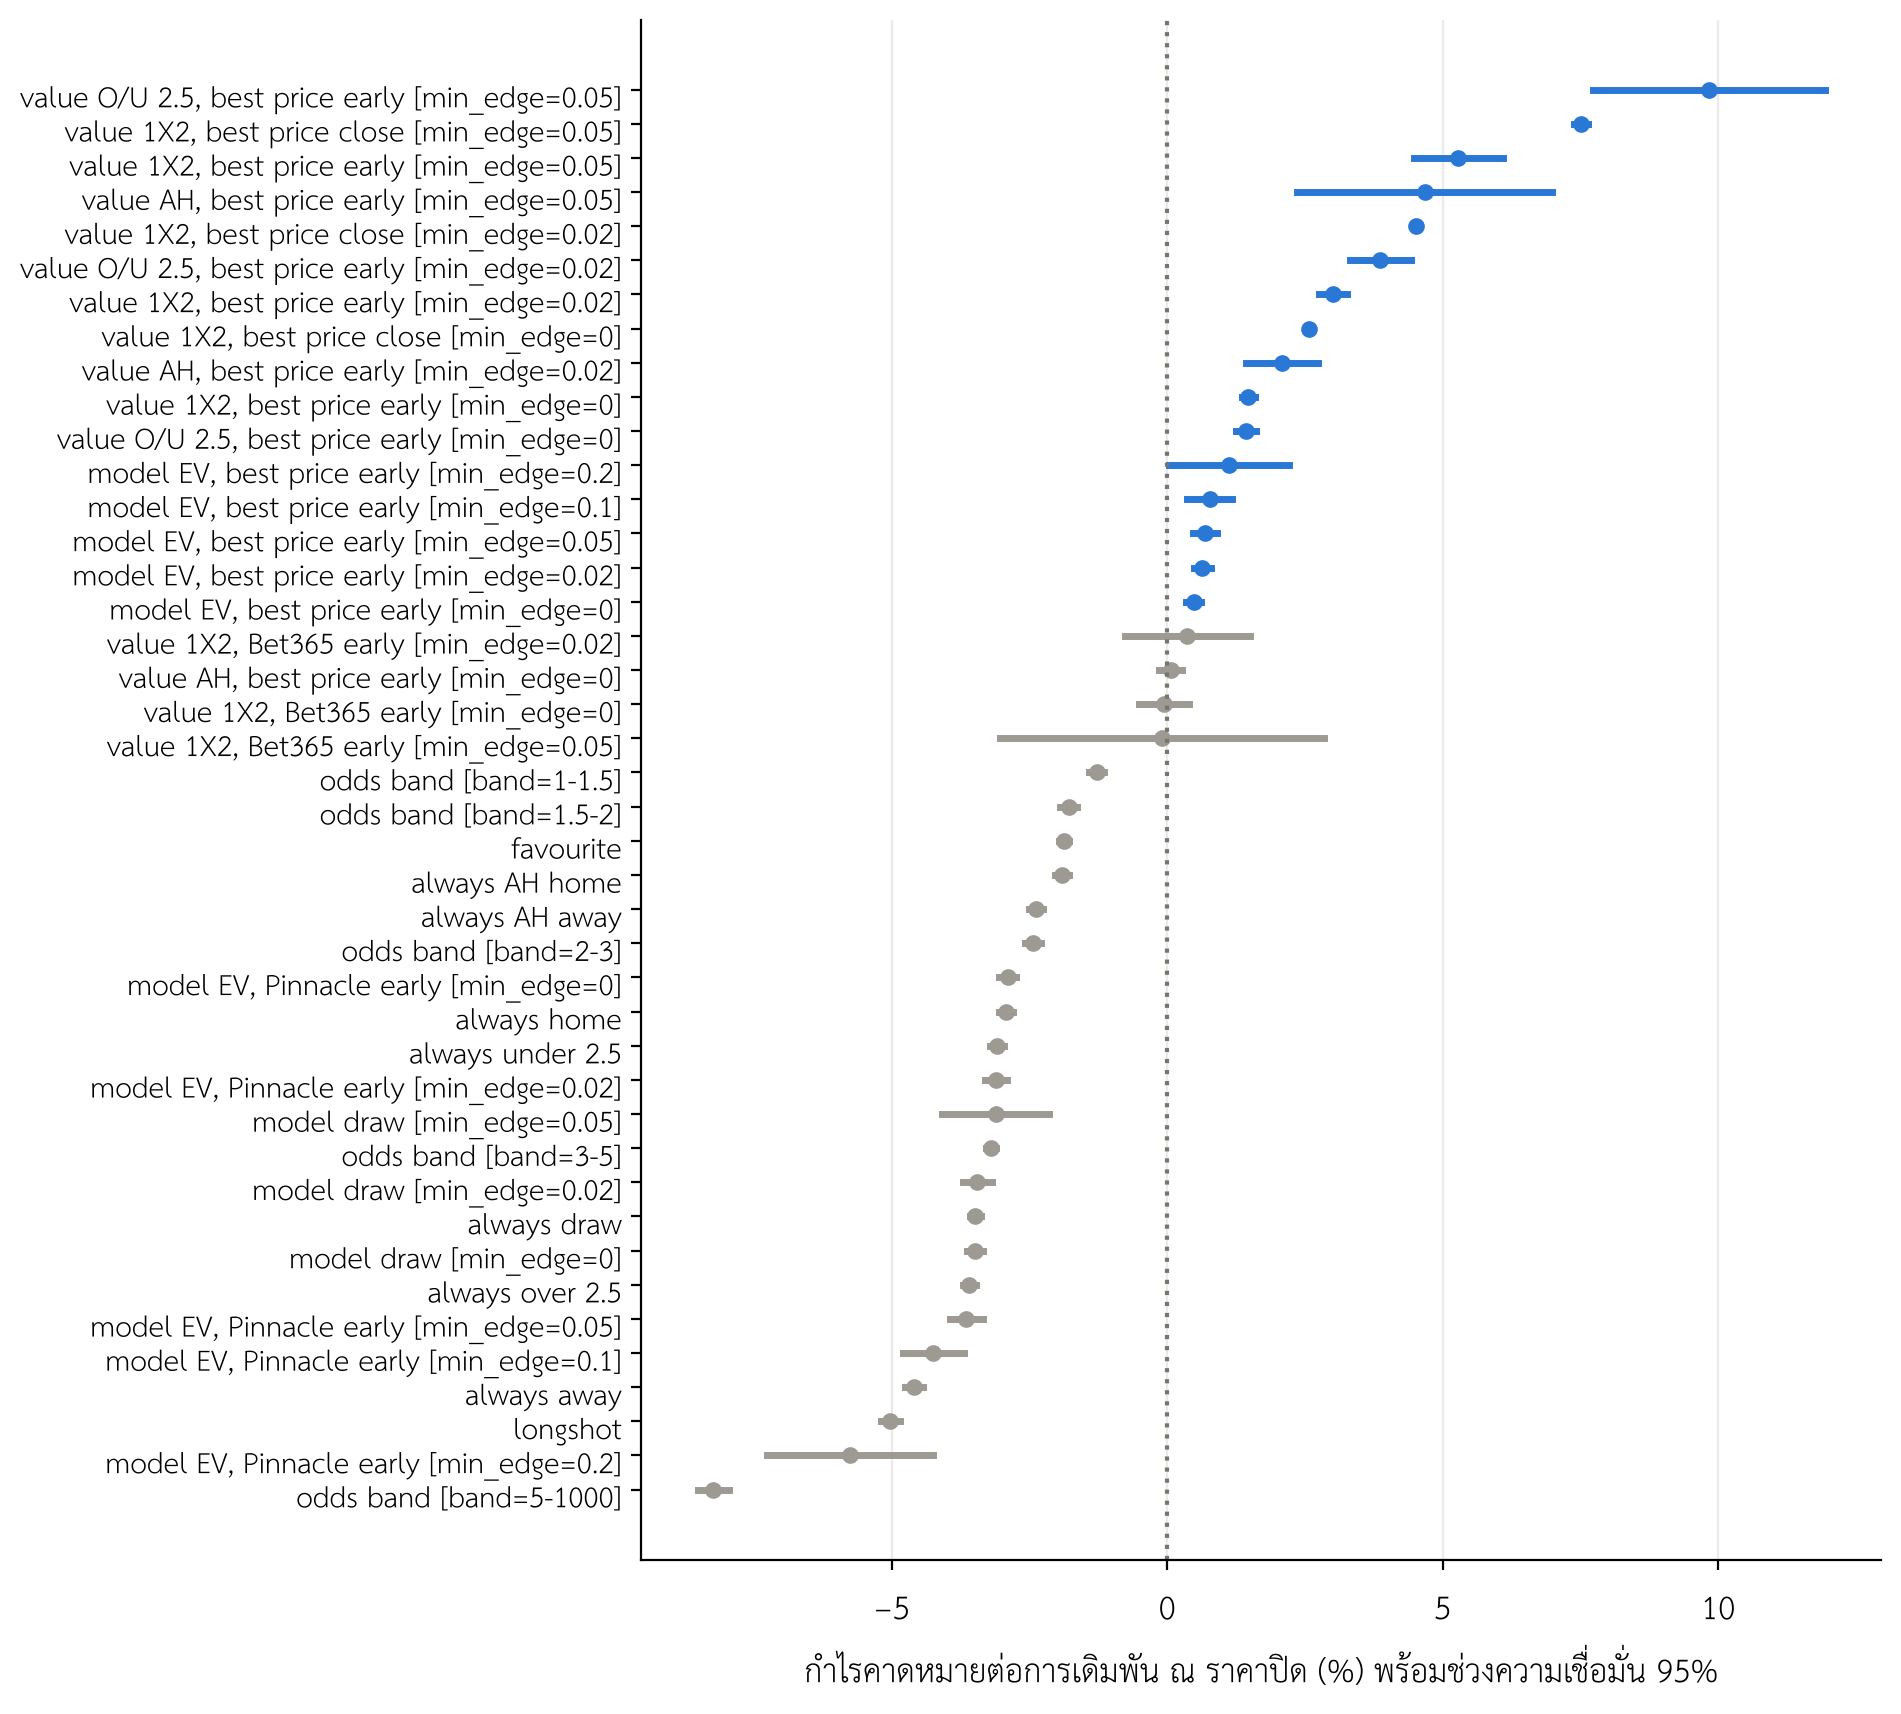
\includegraphics[width=\textwidth]{images/strategy_close_ev.png}
    \caption{กำไรคาดหมายต่อการเดิมพัน ณ ราคาปิด พร้อมช่วงความเชื่อมั่น 95\% ของทุกกลยุทธ์ (รวม 5 ลีก) สีน้ำเงินคือกลยุทธ์ที่ช่วงทั้งหมดอยู่เหนือศูนย์}
    \label{fig:strategy_close_ev}
\end{figure}

\begin{table}[htbp]
\centering
\caption{ผลของกลยุทธ์ที่สำคัญ (รวม 5 ลีก ฤดูกาล 2016--2025)}
\label{tab:strategy_results}
\small
\begin{tabular}{|>{\raggedright\arraybackslash}p{4.7cm}|r|>{\centering\arraybackslash}p{4.4cm}|>{\centering\arraybackslash}p{2.0cm}|}
\hline
\textbf{กลยุทธ์} & \textbf{เดิมพัน} & \textbf{ROI (ช่วง 95\%)} & \textbf{กำไรคาดหมาย ณ ราคาปิด} \\
\hline
\multicolumn{4}{|l|}{\textit{กลยุทธ์พื้นฐาน (ราคาเปิดของ Pinnacle)}} \\
\hline
แทงทีมต่อ (Favourite) & 17,088 & $-1.1\%$ ($-2.5\%$ ถึง $+0.4\%$) & $-1.9\%$ \\
แทงทีมรอง (Longshot) & 17,125 & $-7.0\%$ ($-10.1\%$ ถึง $-3.8\%$) & $-5.0\%$ \\
แทงเจ้าบ้านทุกนัด & 17,063 & $-4.2\%$ ($-6.3\%$ ถึง $-2.2\%$) & $-2.9\%$ \\
แทงเสมอทุกนัด & 17,063 & $-2.4\%$ ($-5.0\%$ ถึง $+0.3\%$) & $-3.5\%$ \\
แทงทีมเยือนทุกนัด & 17,063 & $-5.8\%$ ($-8.5\%$ ถึง $-3.0\%$) & $-4.6\%$ \\
\hline
\multicolumn{4}{|l|}{\textit{กลยุทธ์ตามแบบจำลอง (ราคาเปิด + ฟอร์มทีม)}} \\
\hline
Model EV ที่ราคา Pinnacle ($EV > 2\%$) & 7,793 & $-0.4\%$ ($-4.3\%$ ถึง $+3.6\%$) & $-3.1\%$ \\
Model EV ที่ราคาดีที่สุด ($EV > 2\%$) & 13,665 & $+2.8\%$ ($-0.2\%$ ถึง $+5.8\%$) & $+0.6\%$ \\
Model Draw (ขอบ $> 0$) & 9,821 & $+0.1\%$ ($-3.4\%$ ถึง $+3.7\%$) & $-3.5\%$ \\
\hline
\multicolumn{4}{|l|}{\textit{Value Betting ที่ราคาดีที่สุดเทียบกับ Pinnacle (Line Shopping)}} \\
\hline
1X2 ราคาเปิด (ขอบ $> 2\%$) & 6,240 & $+2.3\%$ ($-2.2\%$ ถึง $+6.8\%$) & $+3.0\%$ \\
1X2 ราคาปิด (ขอบ $> 5\%$) & 2,230 & $+8.1\%$ ($-1.0\%$ ถึง $+17.3\%$) & $+7.5\%$ \\
Over/Under 2.5 ราคาเปิด (ขอบ $> 2\%$) & 668 & $+5.5\%$ ($-2.4\%$ ถึง $+13.3\%$) & $+3.9\%$ \\
Asian Handicap ราคาเปิด (ขอบ $> 2\%$) & 644 & $+5.9\%$ ($-1.0\%$ ถึง $+12.8\%$) & $+2.1\%$ \\
\hline
\end{tabular}
\end{table}

ผลจากภาพที่ \ref{fig:strategy_close_ev} และตารางที่ \ref{tab:strategy_results} สรุปได้ดังนี้
\begin{enumerate}[label=\arabic*)]
    \item \textbf{ไม่มีกลยุทธ์ใดผ่านการปรับแก้การทดสอบหลายครั้ง:} จาก 252 ช่อง ไม่มีช่องใดมีค่า $q$-value ต่ำกว่า $0.05$ (ทุกช่องมีค่า $q \approx 1.00$) ROI ที่เป็นบวกทุกค่าจึงอธิบายได้ด้วยความบังเอิญ
    \item \textbf{กลยุทธ์ง่าย ๆ ขาดทุนตามส่วนต่างของเจ้ามือ:} ROI อยู่ระหว่าง $-7.0\%$ ถึง $-1.1\%$ โดยการแทงทีมรองขาดทุนมากที่สุด สอดคล้องกับปรากฏการณ์ Favourite--Longshot Bias
    \item \textbf{แบบจำลองไม่มีความได้เปรียบที่ราคา Pinnacle:} เมื่อวางเดิมพันที่ราคาเดียวกับตลาดที่แบบจำลองใช้ กำไรคาดหมาย ณ ราคาปิดติดลบทุกเกณฑ์ ($-2.9\%$ ถึง $-5.8\%$) ส่วนเวอร์ชันที่ราคาดีที่สุดมีกำไรคาดหมายบวกเล็กน้อย ($+0.5\%$ ถึง $+1.1\%$) ซึ่งมาจากการเลือกราคา ไม่ใช่จากแบบจำลอง
    \item \textbf{กลุ่มเดียวที่มีความได้เปรียบตามคาดหมายคือ Line Shopping:} การวางเดิมพันที่ราคาดีที่สุดในบรรดาเจ้ามือเมื่อราคานั้นสูงกว่าความน่าจะเป็นของ Pinnacle ตามแนวทางของ Kaunitz และคณะ \cite{kaunitz2017beating} มีกำไรคาดหมาย ณ ราคาปิด $+1.4\%$ ถึง $+9.8\%$ ต่อการเดิมพัน และช่วงความเชื่อมั่นอยู่เหนือศูนย์ทั้งหมด (ยกเว้น Asian Handicap ที่ขอบ $0$ ซึ่งได้ $+0.1\%$ และช่วงคร่อมศูนย์) แต่ ROI ที่เกิดขึ้นจริงยังมีช่วงความเชื่อมั่นคร่อมศูนย์
\end{enumerate}

เมื่อเลือกพารามิเตอร์ของแต่ละฤดูกาลจากฤดูกาลก่อนหน้าเท่านั้น (Walk-forward) ผลยังเป็นทิศทางเดียวกัน กลยุทธ์ที่ดีที่สุดที่มีจำนวนเดิมพันมากพอ คือ Model EV ที่ราคาดีที่สุด ได้ ROI $+2.7\%$ ($-0.5\%$ ถึง $+5.9\%$ จาก 11,971 เดิมพัน) ซึ่งยังไม่มีนัยสำคัญ

% -----------------------------------------------------------
\section{ผลของกลยุทธ์การบริหารเงินทุน (Staking)}
% -----------------------------------------------------------

นำเดิมพันของกลยุทธ์ตัวแทนมาเล่นซ้ำตามลำดับวันที่ เริ่มจากเงินทุน 1 หน่วย ด้วยแผนการวางเงิน 5 แบบ ได้แก่ เงินคงที่ 1\% ของทุนเริ่มต้น (Flat), Kelly เต็ม, Half Kelly, Quarter Kelly และ Martingale (เบิ้ลเงินเป็น 2 เท่าหลังแพ้) จากนั้นสุ่มเดิมพันแบบมีการแทนที่ (Bootstrap) สร้างประวัติจำลอง 1,000 ชุด ยาว 1, 3 และ 5 ฤดูกาล เพื่อวัดโอกาสที่เงินทุนจะลดลงครึ่งหนึ่ง (ตารางแสดงผลของประวัติ 3 ฤดูกาล) ผลแสดงดังตารางที่ \ref{tab:staking}

\begin{table}[htbp]
\centering
\caption{ผลของแผนการวางเงิน: เงินทุนสุดท้ายในประวัติจริง และโอกาสเสียเงินทุนครึ่งหนึ่งในประวัติจำลอง 3 ฤดูกาล}
\label{tab:staking}
\small
\begin{tabular}{|p{3.0cm}|>{\centering\arraybackslash}p{2.0cm}|>{\centering\arraybackslash}p{2.2cm}|>{\centering\arraybackslash}p{2.2cm}|>{\centering\arraybackslash}p{2.6cm}|}
\hline
\textbf{แผนวางเงิน} & \textbf{ทุนสุดท้าย} & \textbf{Drawdown สูงสุด} & \textbf{โอกาสเสียครึ่ง} & \textbf{ค่ามัธยฐาน ทุนสุดท้าย} \\
\hline
\multicolumn{5}{|l|}{\textit{แทงทีมต่อ}} \\
\hline
Flat & $0.01\times$ & $100\%$ & $75\%$ & $0.39\times$ \\
Martingale & $0.00\times$ & $100\%$ & $96\%$ & $0.00\times$ \\
\hline
\multicolumn{5}{|l|}{\textit{Model EV ราคา Pinnacle}} \\
\hline
Flat & $0.71\times$ & $97\%$ & $59\%$ & $0.84\times$ \\
Kelly & $0.01\times$ & $99\%$ & $95\%$ & $0.05\times$ \\
Quarter Kelly & $0.53\times$ & $72\%$ & $37\%$ & $0.79\times$ \\
\hline
\multicolumn{5}{|l|}{\textit{Model EV ราคาดีที่สุด}} \\
\hline
Flat & $4.80\times$ & $48\%$ & $35\%$ & $2.03\times$ \\
Kelly & $0.01\times$ & $100\%$ & $89\%$ & $0.22\times$ \\
Half Kelly & $25.84\times$ & $89\%$ & $56\%$ & $2.47\times$ \\
Quarter Kelly & $20.64\times$ & $61\%$ & $18\%$ & $2.39\times$ \\
\hline
\multicolumn{5}{|l|}{\textit{Value 1X2 ราคาดีที่สุด}} \\
\hline
Flat & $2.43\times$ & $42\%$ & $31\%$ & $1.47\times$ \\
Kelly & $53.06\times$ & $87\%$ & $34\%$ & $3.34\times$ \\
Quarter Kelly & $4.87\times$ & $36\%$ & $0\%$ & $1.61\times$ \\
Martingale & $0.00\times$ & $100\%$ & $99\%$ & $0.00\times$ \\
\hline
\end{tabular}
\end{table}

ผลที่สำคัญมีดังนี้
\begin{enumerate}[label=\arabic*)]
    \item \textbf{Martingale พาหมดตัวทุกกรณี:} ไม่ว่าจะใช้กับกลยุทธ์ใด (รวมถึงกลยุทธ์ที่มีกำไรคาดหมายเป็นบวก) เงินทุนในประวัติจริงเหลือ $0.00\times$ และในประวัติจำลองเงินทุนลดลงครึ่งหนึ่งภายในฤดูกาลเดียวใน $88\%$ ถึง $100\%$ ของกรณี ($96\%$ ถึง $100\%$ เมื่อจำลอง 3 ฤดูกาล) เพราะการเบิ้ลเงินไม่ได้เปลี่ยนค่าคาดหมายติดลบ แต่ทำให้ขนาดเดิมพันโตจนเกินทุนในช่วงแพ้ติดกัน
    \item \textbf{Kelly เต็มอันตรายเมื่อความน่าจะเป็นไม่แม่น:} Kelly เหมาะสมที่สุดเฉพาะเมื่อความน่าจะเป็นถูกต้อง เมื่อใช้กับความน่าจะเป็นของแบบจำลองที่มั่นใจเกินจริง Kelly เต็มวางเงินมากเกินจนทุนเหลือ $0.01\times$ ทั้งในกลยุทธ์ราคา Pinnacle และราคาดีที่สุด
    \item \textbf{Fractional Kelly ลดความเสี่ยงได้ชัดเจน:} สำหรับกลยุทธ์ Model EV ที่ราคาดีที่สุด Quarter Kelly ลดโอกาสเสียทุนครึ่งหนึ่งจาก $89\%$ (Kelly เต็ม) เหลือ $18\%$
    \item \textbf{ไม่มีแผนวางเงินใดเปลี่ยนค่าคาดหมายติดลบให้เป็นบวกได้:} กลยุทธ์ที่ไม่มีความได้เปรียบ (เช่น แทงทีมต่อ) ขาดทุนเมื่อวางเงินคงที่ ส่วน Kelly ไม่วางเงินเลย (ทุนคงที่ $1.00\times$) เพราะมองไม่เห็นความได้เปรียบที่ราคาของ Pinnacle เอง
\end{enumerate}

% -----------------------------------------------------------
\section{ความเป็นไปได้ในการนำความได้เปรียบไปใช้จริง}
% -----------------------------------------------------------

แม้ Line Shopping จะมีกำไรคาดหมายเป็นบวก แต่การเก็บความได้เปรียบนี้ในทางปฏิบัติมีข้อจำกัด 3 ด้าน

\par\noindent\textbf{1) ระยะเวลากว่าความได้เปรียบจะปรากฏเป็นกำไร}\par\nopagebreak[4]
ผลการแข่งขันฟุตบอลมีความแปรปรวนสูง (ส่วนเบี่ยงเบนมาตรฐาน $\sigma$ ประมาณ 1.8 หน่วยต่อการเดิมพัน 1 หน่วยในตลาด 1X2 และต่ำกว่านี้ในตลาด Over/Under และ Asian Handicap ที่ราคาใกล้ 2.0) ตารางที่ \ref{tab:practicality_time} แสดงจำนวนฤดูกาลที่ต้องเดิมพันทั้ง 5 ลีก กว่ากำไรตามขนาดความได้เปรียบที่คาดหมาย $\mu$ จะสูงกว่าศูนย์ 2 เท่าของความคลาดเคลื่อนมาตรฐาน คือต้องใช้ $n \ge (2\sigma/\mu)^2$ เดิมพัน โดย $\sigma$ คำนวณแยกตามผลกำไรจริงของแต่ละกลยุทธ์

\begin{table}[htbp]
\centering
\caption{จำนวนฤดูกาลที่ต้องเดิมพันกว่าความได้เปรียบจะปรากฏเป็นกำไร (5 ลีก)}
\label{tab:practicality_time}
\small
\begin{tabular}{|>{\raggedright\arraybackslash}p{5.2cm}|>{\centering\arraybackslash}p{1.6cm}|>{\centering\arraybackslash}p{2.3cm}|>{\centering\arraybackslash}p{1.6cm}|>{\centering\arraybackslash}p{1.7cm}|}
\hline
\textbf{กลยุทธ์} & \textbf{เดิมพัน/ฤดูกาล} & \textbf{กำไรคาดหมาย ณ ราคาปิด} & \textbf{หน่วย/ฤดูกาล} & \textbf{ฤดูกาลที่ต้องใช้} \\
\hline
Value 1X2 ราคาปิด (ขอบ $> 2\%$) & 1,040 & $+4.5\%$ & 47 & 6 \\
Value 1X2 ราคาเปิด (ขอบ $> 2\%$) & 624 & $+3.0\%$ & 19 & 23 \\
Value O/U 2.5 ราคาเปิด (ขอบ $> 2\%$) & 95 & $+3.9\%$ & 4 & 30 \\
Value AH ราคาเปิด (ขอบ $> 2\%$) & 92 & $+2.1\%$ & 2 & 81 \\
Model EV ราคาดีที่สุด ($EV > 2\%$) & 1,366 & $+0.6\%$ & 9 & 226 \\
\hline
\end{tabular}
\end{table}

\par\noindent\textbf{2) การปิดบัญชีของเจ้ามือ}\par\nopagebreak[4]
ราคาดีที่สุดมักมาจากเจ้ามือทั่วไป (Soft Bookmakers) ซึ่งจำกัดหรือปิดบัญชีของผู้ที่ชนะ ตามที่ Kaunitz และคณะ \cite{kaunitz2017beating} พบเมื่อทดลองด้วยเงินจริง การจำลองกระจายเดิมพันของกลยุทธ์ Value 1X2 ราคาเปิด ไปยังบัญชีหลายบัญชี โดยปิดบัญชีเมื่อกำไรถึงเกณฑ์ พบว่าถ้ามี 5 บัญชีและถูกปิดเมื่อกำไร 5 หน่วย จะวางเดิมพันได้เพียง 1,108 จาก 6,240 ครั้ง ได้กำไร $+32$ หน่วย และบัญชีสุดท้ายถูกปิดตั้งแต่เดือนกันยายน 2017 ส่วนกรณีที่ดีที่สุด (10 บัญชี ปิดเมื่อกำไร 20 หน่วย) ได้กำไร $+246$ หน่วยก่อนถูกปิดทั้งหมดในเดือนตุลาคม 2021

\par\noindent\textbf{3) ตลาดแลกเปลี่ยน (Betting Exchange)}\par\nopagebreak[4]
Betfair Exchange ไม่ปิดบัญชีผู้ชนะ แต่เก็บค่าคอมมิชชันจากกำไรสุทธิ เมื่อใช้กฎเดียวกันที่ราคา Exchange (ข้อมูลฤดูกาล 2024--2025) ได้ ROI $-18.0\%$ จาก 318 เดิมพันเมื่อค่าคอมมิชชัน 2\% และ $-25.9\%$ จาก 110 เดิมพันเมื่อค่าคอมมิชชัน 5\% โดยกำไรคาดหมาย ณ ราคาปิดเท่ากับ $0.0\%$ และ $-1.1\%$ ตามลำดับ ความได้เปรียบจึงไม่มีอยู่ในตลาดที่ไม่ปิดบัญชีผู้ชนะ

% -----------------------------------------------------------
\section{สรุปผลการวิเคราะห์}
% -----------------------------------------------------------

\begin{enumerate}[label=\arabic*)]
    \item ความได้เปรียบของเจ้าบ้าน ($+0.362$ ประตูต่อนัด) และความสัมพันธ์ระหว่าง Elo กับผลต่างประตู ($r = 0.441$) มีนัยสำคัญทางสถิติ
    \item ตัวแปรที่ช่วยทำนายได้จริงคือ คะแนน Elo, ฟอร์มผู้เล่นตัวจริง, จำนวนนัดใน 14 วัน และนาทีลงเล่นก่อนหน้า ส่วนดัชนีความเหนื่อยล้าไม่ได้ช่วยเมื่อมี Elo อยู่แล้ว
    \item Logistic Regression ดีที่สุดในบรรดาแบบจำลองที่ทดสอบ (Log Loss $0.9855$, Accuracy $52.41\%$) แต่ยังด้อยกว่าราคาเจ้ามือ ($0.9691$)
    \item การวางเดิมพันตามแบบจำลองที่ราคาตลาดขาดทุนประมาณ $4$--$5.5\%$ ทุกเกณฑ์ $EV$ และไม่มีกลยุทธ์ใดใน 252 ช่องที่มีนัยสำคัญหลังปรับแก้การทดสอบหลายครั้ง
    \item ความได้เปรียบตามคาดหมายมีเฉพาะ Line Shopping แต่ต้องใช้เวลาหลายฤดูกาลกว่าจะเห็นเป็นกำไร เจ้ามือที่ให้ราคานั้นปิดบัญชีผู้ชนะ และหายไปในตลาดแลกเปลี่ยน
    \item Martingale และ Kelly เต็มพาเงินทุนหมดได้ง่าย ส่วน Fractional Kelly ลดความเสี่ยงได้แต่ไม่สร้างความได้เปรียบ
\end{enumerate}
